% Options for packages loaded elsewhere
\PassOptionsToPackage{unicode}{hyperref}
\PassOptionsToPackage{hyphens}{url}
%
\documentclass[
]{book}
\usepackage{amsmath,amssymb}
\usepackage{iftex}
\ifPDFTeX
  \usepackage[T1]{fontenc}
  \usepackage[utf8]{inputenc}
  \usepackage{textcomp} % provide euro and other symbols
\else % if luatex or xetex
  \usepackage{unicode-math} % this also loads fontspec
  \defaultfontfeatures{Scale=MatchLowercase}
  \defaultfontfeatures[\rmfamily]{Ligatures=TeX,Scale=1}
\fi
\usepackage{lmodern}
\ifPDFTeX\else
  % xetex/luatex font selection
\fi
% Use upquote if available, for straight quotes in verbatim environments
\IfFileExists{upquote.sty}{\usepackage{upquote}}{}
\IfFileExists{microtype.sty}{% use microtype if available
  \usepackage[]{microtype}
  \UseMicrotypeSet[protrusion]{basicmath} % disable protrusion for tt fonts
}{}
\makeatletter
\@ifundefined{KOMAClassName}{% if non-KOMA class
  \IfFileExists{parskip.sty}{%
    \usepackage{parskip}
  }{% else
    \setlength{\parindent}{0pt}
    \setlength{\parskip}{6pt plus 2pt minus 1pt}}
}{% if KOMA class
  \KOMAoptions{parskip=half}}
\makeatother
\usepackage{xcolor}
\usepackage{color}
\usepackage{fancyvrb}
\newcommand{\VerbBar}{|}
\newcommand{\VERB}{\Verb[commandchars=\\\{\}]}
\DefineVerbatimEnvironment{Highlighting}{Verbatim}{commandchars=\\\{\}}
% Add ',fontsize=\small' for more characters per line
\usepackage{framed}
\definecolor{shadecolor}{RGB}{248,248,248}
\newenvironment{Shaded}{\begin{snugshade}}{\end{snugshade}}
\newcommand{\AlertTok}[1]{\textcolor[rgb]{0.94,0.16,0.16}{#1}}
\newcommand{\AnnotationTok}[1]{\textcolor[rgb]{0.56,0.35,0.01}{\textbf{\textit{#1}}}}
\newcommand{\AttributeTok}[1]{\textcolor[rgb]{0.13,0.29,0.53}{#1}}
\newcommand{\BaseNTok}[1]{\textcolor[rgb]{0.00,0.00,0.81}{#1}}
\newcommand{\BuiltInTok}[1]{#1}
\newcommand{\CharTok}[1]{\textcolor[rgb]{0.31,0.60,0.02}{#1}}
\newcommand{\CommentTok}[1]{\textcolor[rgb]{0.56,0.35,0.01}{\textit{#1}}}
\newcommand{\CommentVarTok}[1]{\textcolor[rgb]{0.56,0.35,0.01}{\textbf{\textit{#1}}}}
\newcommand{\ConstantTok}[1]{\textcolor[rgb]{0.56,0.35,0.01}{#1}}
\newcommand{\ControlFlowTok}[1]{\textcolor[rgb]{0.13,0.29,0.53}{\textbf{#1}}}
\newcommand{\DataTypeTok}[1]{\textcolor[rgb]{0.13,0.29,0.53}{#1}}
\newcommand{\DecValTok}[1]{\textcolor[rgb]{0.00,0.00,0.81}{#1}}
\newcommand{\DocumentationTok}[1]{\textcolor[rgb]{0.56,0.35,0.01}{\textbf{\textit{#1}}}}
\newcommand{\ErrorTok}[1]{\textcolor[rgb]{0.64,0.00,0.00}{\textbf{#1}}}
\newcommand{\ExtensionTok}[1]{#1}
\newcommand{\FloatTok}[1]{\textcolor[rgb]{0.00,0.00,0.81}{#1}}
\newcommand{\FunctionTok}[1]{\textcolor[rgb]{0.13,0.29,0.53}{\textbf{#1}}}
\newcommand{\ImportTok}[1]{#1}
\newcommand{\InformationTok}[1]{\textcolor[rgb]{0.56,0.35,0.01}{\textbf{\textit{#1}}}}
\newcommand{\KeywordTok}[1]{\textcolor[rgb]{0.13,0.29,0.53}{\textbf{#1}}}
\newcommand{\NormalTok}[1]{#1}
\newcommand{\OperatorTok}[1]{\textcolor[rgb]{0.81,0.36,0.00}{\textbf{#1}}}
\newcommand{\OtherTok}[1]{\textcolor[rgb]{0.56,0.35,0.01}{#1}}
\newcommand{\PreprocessorTok}[1]{\textcolor[rgb]{0.56,0.35,0.01}{\textit{#1}}}
\newcommand{\RegionMarkerTok}[1]{#1}
\newcommand{\SpecialCharTok}[1]{\textcolor[rgb]{0.81,0.36,0.00}{\textbf{#1}}}
\newcommand{\SpecialStringTok}[1]{\textcolor[rgb]{0.31,0.60,0.02}{#1}}
\newcommand{\StringTok}[1]{\textcolor[rgb]{0.31,0.60,0.02}{#1}}
\newcommand{\VariableTok}[1]{\textcolor[rgb]{0.00,0.00,0.00}{#1}}
\newcommand{\VerbatimStringTok}[1]{\textcolor[rgb]{0.31,0.60,0.02}{#1}}
\newcommand{\WarningTok}[1]{\textcolor[rgb]{0.56,0.35,0.01}{\textbf{\textit{#1}}}}
\usepackage{longtable,booktabs,array}
\usepackage{calc} % for calculating minipage widths
% Correct order of tables after \paragraph or \subparagraph
\usepackage{etoolbox}
\makeatletter
\patchcmd\longtable{\par}{\if@noskipsec\mbox{}\fi\par}{}{}
\makeatother
% Allow footnotes in longtable head/foot
\IfFileExists{footnotehyper.sty}{\usepackage{footnotehyper}}{\usepackage{footnote}}
\makesavenoteenv{longtable}
\usepackage{graphicx}
\makeatletter
\def\maxwidth{\ifdim\Gin@nat@width>\linewidth\linewidth\else\Gin@nat@width\fi}
\def\maxheight{\ifdim\Gin@nat@height>\textheight\textheight\else\Gin@nat@height\fi}
\makeatother
% Scale images if necessary, so that they will not overflow the page
% margins by default, and it is still possible to overwrite the defaults
% using explicit options in \includegraphics[width, height, ...]{}
\setkeys{Gin}{width=\maxwidth,height=\maxheight,keepaspectratio}
% Set default figure placement to htbp
\makeatletter
\def\fps@figure{htbp}
\makeatother
\setlength{\emergencystretch}{3em} % prevent overfull lines
\providecommand{\tightlist}{%
  \setlength{\itemsep}{0pt}\setlength{\parskip}{0pt}}
\setcounter{secnumdepth}{5}
\usepackage{booktabs}
\ifLuaTeX
  \usepackage{selnolig}  % disable illegal ligatures
\fi
\usepackage[]{natbib}
\bibliographystyle{apalike}
\IfFileExists{bookmark.sty}{\usepackage{bookmark}}{\usepackage{hyperref}}
\IfFileExists{xurl.sty}{\usepackage{xurl}}{} % add URL line breaks if available
\urlstyle{same}
\hypersetup{
  pdftitle={Stat 220 Introduction to Data Science},
  pdfauthor={Deepak Bastola},
  hidelinks,
  pdfcreator={LaTeX via pandoc}}

\title{Stat 220 Introduction to Data Science}
\author{Deepak Bastola}
\date{2024-03-20}

\begin{document}
\maketitle

{
\setcounter{tocdepth}{1}
\tableofcontents
}
\hypertarget{course-overview}{%
\chapter*{Course overview}\label{course-overview}}
\addcontentsline{toc}{chapter}{Course overview}

Greetings and welcome to Introduction to Data Science! In this course, we will delve into the computational aspects of data analysis, covering topics such as data acquisition, management, and visualization tools. Throughout this course, we will emphasize the principles of data-scientific, reproducible research and dynamic programming, utilizing the R/RStudio ecosystem.

If you have taken Stat 120, 230, or 250 at Carleton, you will find yourself well-equipped to handle the material. However, it is important to refresh your R and R-markdown skills before the start of the class. Specifically, I expect all students to be able to load a data set into R, calculate basic summary statistics, and perform basic exploratory data analysis. In the first week of class, we will delve into Git and GitHub version control, though prior exposure to these topics is not necessary.

\hypertarget{learning-objectives}{%
\section{Learning Objectives}\label{learning-objectives}}

\begin{itemize}
\tightlist
\item
  Develop research questions that can be answered by data. Import/scrape data into R and reshape it to the form necessary for analysis.
\item
  Manipulate common types of data, including numeric, categorical (factors), text, date-times, geo-location variables in order to provide insight into your data and facilitate analysis.
\item
  Explore data using both graphical and numeric methods to provide insight and uncover relationships/patterns.
\item
  Utilize fundamental programming concepts such as iteration, conditional execution, and functions to streamline your code.
\item
  Build, tune, use, and evaluate basic statistical learning models to uncover clusters and classify observations.
\item
  Draw informed conclusions from your data and communicate your findings using both written and interactive platforms.
\end{itemize}

\hypertarget{part-set-up-instructions}{%
\part*{Set-up Instructions}\label{part-set-up-instructions}}
\addcontentsline{toc}{part}{Set-up Instructions}

\hypertarget{rstudio}{%
\chapter{What is R, RStudio, and RMarkdown?}\label{rstudio}}

R is a free and open source statistical programming language that facilitates statistical computation. There are a myriad of application that can be done in R, thanks to a huge online support community and dedicated packages. However, R has no graphical user interface and it has to be run by typing commands into a text interface.

\hypertarget{what-is-rstudio}{%
\section{What is RStudio?}\label{what-is-rstudio}}

RStudio provides graphical interface to R! You can think of RStudio as a graphical front-end to R that that provides extra functionality. The use of the R programming language with the RStudio interface is an essential component of this course.

\hypertarget{r-studio-server}{%
\section{R Studio Server}\label{r-studio-server}}

The quickest way to get started is to go to \url{https://maize2.mathcs.carleton.edu}, which opens an R Studio window in your web browser. Once logged in, I recommend that you do the following:

\begin{itemize}
\tightlist
\item
  Step 1: Create a folder for this course where you can save all of your work. In the Files window, click on New Folder.
\item
  Step 2: Click on Tools -\textgreater{} Global Options -\textgreater{} R Markdown. Then uncheck the box that says ``Show output inline\ldots{}''
\end{itemize}

(It is also possible to download RStudio on your own laptop. Instructions may be found at the end of this document.)

\hypertarget{rrstudio}{%
\section{R/RStudio}\label{rrstudio}}

The use of the R programming language with the RStudio interface is an
essential component of this course. You have two options for using
RStudio:

\begin{itemize}
\item
  The \textbf{server version} of RStudio on the web at
  (\url{https://maize2.mathcs.carleton.edu}). The advantage of using the
  server version is that all of your work will be stored in the cloud,
  where it is automatically saved and backed up. This means that you
  can access your work from any computer on campus using a web
  browser. This server may run slow during peak days/hours. I also recommend
  you to download a local version of R server in your computer in case of rare outages.
\item
  A \textbf{local version} of RStudio installed on your machine. This
  option is highly recommended due to the computational resources this
  course demands. Using this version you can only store your files in your local machine. Additionally, we can save our work on GitHub. We will learn how to use GitHub in the beginning of the course. Both R and RStudio are free and open-source. Please make sure that you have recently updated both R and RStudio.
\end{itemize}

\hypertarget{installing-rrstudio-not-needed-if-you-are-using-the-maize-server}{%
\section{\texorpdfstring{\textbf{Installing R/RStudio (not needed if you are using the maize server)}}{Installing R/RStudio (not needed if you are using the maize server)}}\label{installing-rrstudio-not-needed-if-you-are-using-the-maize-server}}

\begin{quote}
Download the latest version of R: \url{https://cran.r-project.org/}
Download the free Rstudio desktop version: \url{https://www.rstudio.com/products/rstudio/download/}
\end{quote}

Use the default download and install options for each. For R, download the ``precompiled binary'' distribution rather than the source code

\textbf{Updating R/RStudio (not needed if you are using the maize server)}

If you have used a local version of R/RStudio before and it is still installed on your machine, then you should make sure that you have the most recent versions of each program.

\begin{itemize}
\item
  To check your version of R, run the command \texttt{getRversion()} and compare your version to the newest version posted on \url{https://cran.r-project.org/}. If you need an update, then install the newer version using the installation directions above.
\item
  In RStudio, check for updates with the menu option \texttt{Help\ \textgreater{}\ Check\ for\ updates}. Follow directions if an update is needed.
\end{itemize}

** Did it work? (A sanity check after your install/update) **

Do whatever is appropriate for your operating system to launch
RStudio. You should get a window similar to the screenshot you see
\href{https://www.rstudio.com/wp-content/uploads/2014/04/rstudio-workbench.png}{here},
but yours will be more boring because you haven't written any code
or made any figures yet!

Put your cursor in the pane labeled \emph{Console}, which is where you
interact with the live R process. Create a simple object with code
like \texttt{x\ \textless{}-\ 2\ *\ 4} (followed by enter or return). Then inspect the
\texttt{x} object by typing \texttt{x} followed by enter or return. You should see
the value \texttt{8} printed. If this happened, you've succeeded in
installing R and RStudio!

\hypertarget{what-is-rmarkdown}{%
\section{What is RMarkdown?}\label{what-is-rmarkdown}}

An R Markdown file (.Rmd file) combines R commands and written analyses, which are `knit' together into an HTML, PDF, or Microsoft Word document.

An R Markdown file contains three essential elements:

\begin{itemize}
\item
  Header: The header (top) of the file contains information like the document title, author, date and your preferred output format (pdf\_document, word\_document, or html\_document).
\item
  Written analysis: You write up your analysis after the header and embed R code where needed. The online help below shows ways to add formatting details like bold words, lists, section labels, etc to your final pdf/word/html document. For example, adding ** before and after a word will bold that word in your compiled document.
\item
  R chunks: R chunks contain the R commands that you want evaluated. You embed these chunks within your written analysis and they are evaluated when you compile the document.
\end{itemize}

\hypertarget{install-latex-for-knitting-r-markdown-documents-to-pdf}{%
\section{Install LaTeX (for knitting R Markdown documents to PDF):}\label{install-latex-for-knitting-r-markdown-documents-to-pdf}}

You need a Latex compiler to create a pdf document from a R Markdown file. If you use the maize server, you don't need to install anything. If you are using a local RStudio, you should install a Latex compiler. Below are the recommended installers for Windows and Mac:

\begin{itemize}
\item
  \href{https://www.tug.org/mactex/}{MacTeX} for Mac (3.2GB)
\item
  \href{https://miktex.org/download}{MiKTeX} for Windows (190MB)
\item
  Alternatively, you can install the \texttt{tinytex} R package by running
  \texttt{install.packages("tinytex")} in the console.
\end{itemize}

\hypertarget{updating-rrstudio-not-needed-if-you-are-using-the-maize2-server}{%
\section{Updating R/RStudio (not needed if you are using the maize2 server)}\label{updating-rrstudio-not-needed-if-you-are-using-the-maize2-server}}

If you have used a local version of R/RStudio before and it is still installed on your machine, then you should make sure that you have the most recent versions of each program.

\begin{itemize}
\item
  To check your version of R, run the command \texttt{getRversion()} and compare your version to the newest version posted on \url{https://cran.r-project.org/}. If you need an update, then install the newer version using the installation directions above.
\item
  In RStudio, check for updates with the menu option \texttt{Help\ \textgreater{}\ Check\ for\ updates}. Follow directions if an update is needed.
\end{itemize}

\hypertarget{opening-a-new-file}{%
\section{Opening a new file}\label{opening-a-new-file}}

If using Rstudio on your computer, using the \textbf{File\textgreater Open File} menu to find and open this .Rmd file.

If using Maize Rstudio from your browser:

\begin{itemize}
\item
  In the Files tab, select \textbf{Upload} and \textbf{Choose File} to find the .Rmd that you downloaded. Click \emph{OK} to upload to your course folder/location in the maize server account.
\item
  Click on the .Rmd file in the appropriate folder to open the file.
\end{itemize}

\hypertarget{running-codes-and-knitting-.rmd-files}{%
\section{Running codes and knitting .Rmd files:}\label{running-codes-and-knitting-.rmd-files}}

\begin{itemize}
\item
  You can run a line of code by placing your cursor in the line of code and clicking \textbf{Run Selected Line(s)}
\item
  You can run an entire chunk by clicking the green triangle on the right side of the code chunk.
\item
  After each small edit or code addition, \textbf{Knit} your Markdown. If you wait until the end to Knit, it will be harder to find errors in your work.
\item
  Format output type: You can use any of pdf\_document, html\_document type, or word\_document type.
\item
  \textbf{Maize users}: You may also need to allow for ``pop-up'' in your web browser when knitting documents.
\end{itemize}

\hypertarget{few-more-instructions}{%
\section{Few More Instructions}\label{few-more-instructions}}

The default setting in Rstudio when you are running chunks is that the ``output'' (numbers, graphs) are
shown \textbf{inline} within the Markdown Rmd. If you prefer to have your plots appear on the right of the console and not below the chunk, then change the settings as follows:

\begin{enumerate}
\def\labelenumi{\arabic{enumi}.}
\tightlist
\item
  Select Tools \textgreater{} Global Options.
\item
  Click the R Markdown section and uncheck (if needed) the option Show output inline for all
  R Markdown documents.
\item
  Click OK.
\end{enumerate}

Now try running R chunks in the .Rmd file to see the difference. You can recheck this box if you prefer
the default setting.

\hypertarget{vpn}{%
\section{VPN}\label{vpn}}

If you plan to do any work off campus this term, you need to install Carleton's VPN. This will allow you to access the \textbf{maize} server (if needed).

\textbf{Installing the GlobalProtect VPN}

Follow the directions \href{https://wiki.carleton.edu/display/itskb/GlobalProtect+VPN}{here} to install VPN.

\hypertarget{assignments}{%
\chapter{Assignments in Stat 220}\label{assignments}}

\hypertarget{dos-and-dont-of-collaboration-for-individual-assignments}{%
\section{Do's and Don't of collaboration for individual assignments}\label{dos-and-dont-of-collaboration-for-individual-assignments}}

\begin{itemize}
\tightlist
\item
  You \emph{can} discuss homework problems with classmates but you must
  write up \textbf{your own} homework solutions and \textbf{do your own work in R
  (no sharing commands or output)}.

  \begin{itemize}
  \tightlist
  \item
    \textbf{Do not share R commands/code in any way}, including, but not
    limited to, sending commands via email, slack, text, or showing
    commands in a shared screen with the intention of showing a
    classmate your solution to a problem.
  \item
    You \textbf{can} share a screen to help troubleshoot a coding problem
    in R.
  \end{itemize}
\item
  You \emph{can} use the following resources to complete your homework:

  \begin{itemize}
  \tightlist
  \item
    Carleton faculty (myself, other math or statistics faculty, etc)
  \item
    discussions with classmates (see above) or knowledgeable friends
  \item
    Carleton resources like stats lab assistants
  \item
    student solutions provided in the back of your student textbook
    or in the student solution manual.
  \end{itemize}
\item
  You \emph{cannot} use any resources other than the ones listed above to
  complete assignments (homework, reports, etc) for this class.
  (e.g.~you cannot use a friend's old assignments or reports, answers
  found on the internet, textbook (instructor) solutions manual, etc.)
\end{itemize}

\hypertarget{examples-that-violate-the-academic-integrity-policy}{%
\subsection{Examples that violate the academic integrity policy}\label{examples-that-violate-the-academic-integrity-policy}}

\begin{itemize}
\tightlist
\item
  sending your .Rmd homework file to another person in the class
\item
  receiving an .Rmd homework file from another person
\item
  sharing a screen and copying code, verbatim, from another person
\item
  sending/receiving R commands
\item
  neglecting to acknowledge classmates with whom you worked with on an
  assignment
\end{itemize}

\hypertarget{format-and-content}{%
\section{Format and Content}\label{format-and-content}}

Submit via GitHub (for most assignments) an organized and correctly
ordered assignment.

\begin{itemize}
\tightlist
\item
  Content: Good data scientists need to do more than just write code;
  they should be able to interpret and explain their analyzes.

  \begin{itemize}
  \tightlist
  \item
    Provide a \textbf{written answer} first, followed by any required R
    code and output.\\
  \item
    Use \textbf{complete sentences} when answering any problem that
    requires an explanation or overall problem summary.
  \end{itemize}
\item
  When including code:

  \begin{itemize}
  \tightlist
  \item
    Be sure to show the natural sequence of work needed to answer
    the problem.
  \item
    Include brief comments explain your code steps.
  \item
    Do not include typos or unnecessary commands/output.
  \item
    Always include code output.
  \end{itemize}
\item
  At the top of each individual assignment \textbf{include the names of
  classmates that you worked with} on all or part of the assignment
  (but each person must write up their assignment on their own)
\end{itemize}

\begin{center}\rule{0.5\linewidth}{0.5pt}\end{center}

\textbf{Disability Accommodations:} Carleton College is committed to
providing equitable access to learning opportunities for all students.
The Disability Services office (Henry House, 107 Union Street) is the
campus office that collaborates with students who have disabilities to
provide and/or arrange reasonable accommodations. If you have, or think
you may have, a disability (e.g., mental health, attentional, learning,
autism spectrum disorders, chronic health, traumatic brain injury and
concussions, vision, hearing, mobility, or speech impairments), please
contact \href{mailto:disability@carleton.edu}{\nolinkurl{disability@carleton.edu}} or call Sam Thayer ('10),
Accessibility Specialist (x4464) or Chris Dallager, Director of
Disability Services (x5250) to arrange a confidential discussion
regarding equitable access and reasonable accommodations.

\textbf{Academic Honesty:} All work that you turn in under your name must
follow Carleton's academic integrity policy. The use of textbook
solution manuals (physical or online solutions), homework, reports or
exams done by past students are not allowed. Look at the College's
\href{https://www.carleton.edu/writing/plagiarism/}{Writing Across the Curriculum} website for
additional guidance on plagiarism and how to avoid plagiarism in their
writing.

\hypertarget{software}{%
\chapter{Software in Stat 220}\label{software}}

You will work with many .Rmd Markdown files in this course. These include class activities, homework template, project helper files etc. To stay organized, I \emph{strongly} suggest you create a \textbf{stat220} folder that contains the following subfolders:

\begin{itemize}
\tightlist
\item
  \textbf{stat220} folder

  \begin{itemize}
  \item
    \textbf{Assignments:} This folder will contain subfolders for each
    assignment. Each assignment subfolder (e.g.~homework1,
    homework2, \ldots) will be a Github connected RStudio project that
    you will create \textbf{once an assignment is posted.}
  \item
    \textbf{Content:} This folder should be used to save any
    non-assignment files (e.g.~slides, examples) for this class. You
    will create this subfolder by creating an RStudio project (see
    step 5 below).
  \end{itemize}
\end{itemize}

To get started with this organization, follow the steps below.

\begin{center}\rule{0.5\linewidth}{0.5pt}\end{center}

\hypertarget{file-organization-using-maize}{%
\section{File organization: Using maize}\label{file-organization-using-maize}}

The server (online) version of Rstudio is run from a unix server. You
can navigate this file system using unix commands, but I assume that
most or all of you will just use Rstudio to access your files on this
server.

\begin{quote}
\textbf{1.} In Rstudio, click the \textbf{Files} \emph{tab} in the lower right-hand
window. Note: this is \textbf{not} the same as the \textbf{File} \emph{menu}
option.
\end{quote}

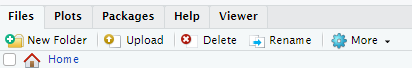
\includegraphics{img/maize_files.png}

\begin{quote}
\textbf{2.} Verify that you are in your \textbf{HOME} folder (should simply
say Home right under the New Folder button). To navigate to your
Home folder (if somehow you are not in it), click the \textbf{\ldots{}} button
(far right side of the \textbf{Files} tab) and enter a \textasciitilde{} (tilde) symbol
\end{quote}

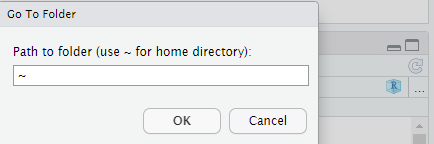
\includegraphics{img/maize_home.png}

\begin{itemize}
\tightlist
\item
  \textbf{3.} Click the \textbf{New Folder} button and name the folder
  \textbf{stat220}.
\end{itemize}

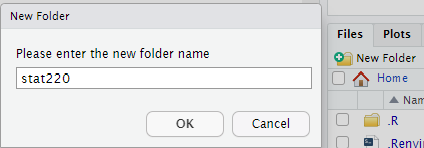
\includegraphics{img/maize_newfolder.png}

\begin{itemize}
\tightlist
\item
  \textbf{4.} Click on this newly created (empty) \textbf{stat220} folder.
  Within the folder create another \textbf{New Folder} and name it
  \textbf{assignments}.
\end{itemize}

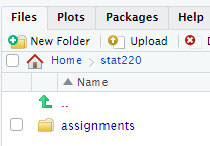
\includegraphics{img/maize_stat220.png}

\begin{itemize}
\item
  \textbf{5.} Within the \textbf{stat220} folder, create an \textbf{RStudio project}
  called \textbf{content} with the following steps:

  \begin{itemize}
  \tightlist
  \item
    \textbf{a.} Click the \textbf{Project} button in the upper righthand
    corner of your RStudio window and select \textbf{New Project\ldots{}}.
  \end{itemize}
\end{itemize}

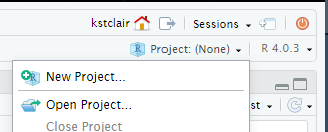
\includegraphics{img/maize_project.png}

\begin{itemize}
\tightlist
\item
  \textbf{b.} Select \textbf{New Directory} and then \textbf{New Project}
\end{itemize}

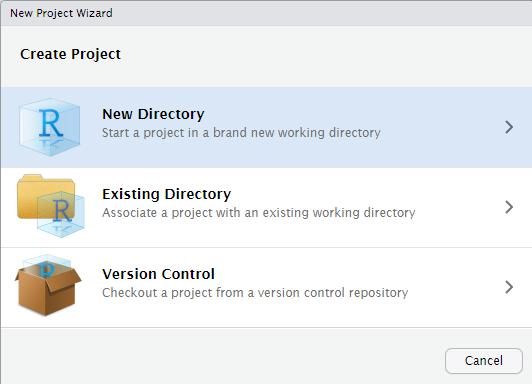
\includegraphics{img/maize_newdirectory.png}

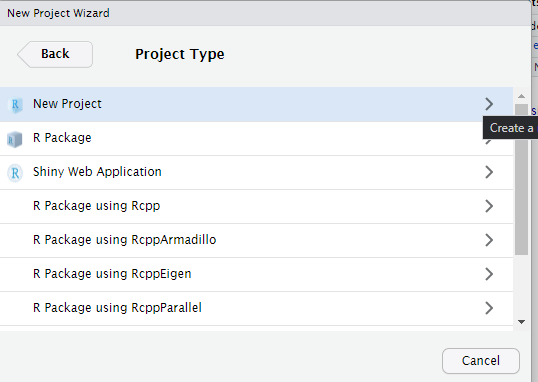
\includegraphics{img/maize_newdirectory2.png}

\begin{itemize}
\tightlist
\item
  \textbf{c.} Enter \textbf{content} as the \textbf{Directory name} and use the
  \textbf{Browse} button to find your \textbf{stat220} folder. Then click
  \textbf{Create Project}.
\end{itemize}

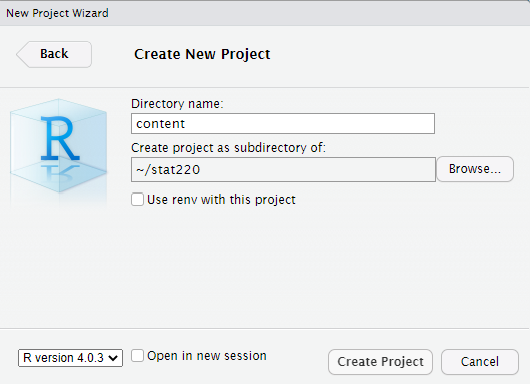
\includegraphics{img/maize_create.png}

\begin{itemize}
\tightlist
\item
  \textbf{d.} You should now have a new folder called \textbf{content} in your
  \textbf{stat220} folder and this folder will contain an RStudio project
  \texttt{.Rproj}. Feel free to add subfolders to this \textbf{content} folder
  (e.g.~slides, examples, etc).
\end{itemize}

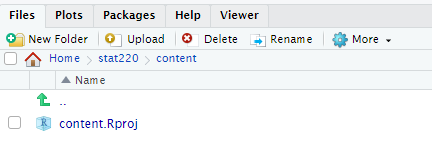
\includegraphics{img/maize_Rproj.png}

\textbf{Warning: Do not} create an RStudio project in the main stat220 folder
because it is not good practice to have RStudio projects in subfolders
of another project (e.g.~a project within a project is not recommended).

\begin{center}\rule{0.5\linewidth}{0.5pt}\end{center}

\hypertarget{file-organization-using-your-own-rstudio}{%
\section{File organization: Using your own Rstudio}\label{file-organization-using-your-own-rstudio}}

Create a folder called \textbf{stat220} somewhere on your computer. Within
this folder create an \textbf{assignments} subfolder. Then complete \textbf{step
5} from above to create a \textbf{content} RStudio project folder.

\begin{center}\rule{0.5\linewidth}{0.5pt}\end{center}

\hypertarget{rstudio-projects}{%
\section{RStudio projects}\label{rstudio-projects}}

Once you've created a project, your R session should be running within
that project folder. You can check which project you are in by checking
the project name in the upper righthand part of your RStudio window.
Here we see the \textbf{content} project is open:

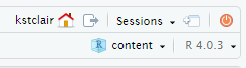
\includegraphics{img/maize_content.png}

Running R from an RStudio project sets your \textbf{working directory} to the
project folder:

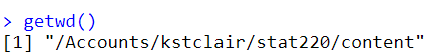
\includegraphics{img/maize_getwd.png}

This allows for easy file path access to all files related to this
project.

To \textbf{start} a project, click on the \texttt{.Rproj} file or use the \textbf{Open
Project\ldots{}} option shown in step 5 above.

\begin{center}\rule{0.5\linewidth}{0.5pt}\end{center}

\hypertarget{best-practices-or-what-not-to-do}{%
\section{Best practices (or what not to do)}\label{best-practices-or-what-not-to-do}}

\begin{itemize}
\tightlist
\item
  Never save files to a lab computer hard drive (e.g.~desktop,
  downloads, etc). They will be erased when you log off.
\item
  Do not use gmail as a file storage system! Avoid emailing yourself
  files that you created (and saved) on a lab computer. Eventually you
  will lose work this way.
\item
  Avoid using online versions of google drive and dropbox. Similar to
  gmail, downloading, editing a doc, then uploading it back to
  drive/dropbox is another great way to lose work.
\item
  Avoid \href{https://xkcd.com/1459/}{this} and \href{http://phdcomics.com/comics.php?f=1531}{this}.
\end{itemize}

\hypertarget{git-and-github}{%
\section{Git and GitHub}\label{git-and-github}}

\href{https://happygitwithr.com/big-picture.html\#why-git}{Git} is version
control software that you install locally on your computer. Git is
already installed on the maize RStudio server.

\href{https://happygitwithr.com/big-picture.html\#why-github}{Github} is a
cloud-based service for hosting git projects. It allows multiple users
to share and contribute to projects and it is how you will be submitting
homework assignments and projects for this class. More information about Git and
Github can also be found in \href{https://rfortherestofus.com/2021/02/how-to-use-git-github-with-r/}{Getting setup with Git and
GitHub} and \href{https://sahirbhatnagar.com/rpkg/\#gitgithub}{Git and Github}.

If you are using a local install of R/RStudio, then you will need to
install Git.

\textbf{Installing Git}

Directions for both Windows \& Mac here:
\url{http://happygitwithr.com/install-git.html}.

\begin{quote}
\begin{enumerate}
\def\labelenumi{\arabic{enumi}.}
\tightlist
\item
  If you are using \textbf{maize}, then there is nothing you need to install.
\item
  Windows users should follow Option 1 in 6.2.
\item
  Mac users can follow Option 1 in 6.3 if comfortable, otherwise follow Option 2
\item
  Linux users can follow 6.4.
\end{enumerate}
\end{quote}

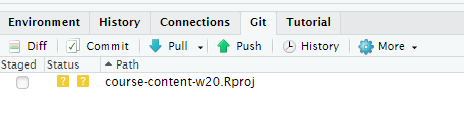
\includegraphics{img/maize_gittab.png}

\hypertarget{slack}{%
\section{Slack}\label{slack}}

We will use Slack for all course communication. \href{https://join.slack.com/t/datasciencewinter24/shared_invite/zt-2a2xv06eo-csIThOBrnJ_UY~jImBiUoQ}{Sign up for our course
Slack team
here}!
You will need to create an account with a username, and log in to read
and post. You can download a
standalone Slack application to your
\href{https://slack.com/downloads/osx}{Mac},
\href{https://slack.com/downloads/windows}{Windows},
\href{https://slack.com/downloads/linux}{Linux} and/or
\href{https://slack.com/downloads/android}{Android}/\href{https://slack.com/downloads/ios}{iOS}
device. You can control whether you receive notifications on new posts
by going to Preferences, as well as decide which `channels' to subscribe
to. A `channel' is a discussion thread, which is used to organize
communications into topics. You can learn more about Slack features
\href{https://slack.com/help/articles/218080037-Getting-started-for-new-Slack-users}{here}.

Several channels have been set up for specific parts of the course. Feel
free to ask questions anytime. You can browse the available channels in
our team by clicking on ``Channels'' on the left-hand panel.

\hypertarget{acknowledgements}{%
\section{Acknowledgements}\label{acknowledgements}}

This installation guide is based on the guide from Adam Loy and Katie St.~Clair.

\hypertarget{github}{%
\chapter{GitHub Guide for Students in Stat 220}\label{github}}

\hypertarget{overview}{%
\section{Overview}\label{overview}}

If you are using the maize RStudio server, then you can connect to
GitHub without any extra software downloads. If you are using RStudio on
your computer, then you will need to download Git software (as directed
in \protect\hyperlink{software}{Software in Stat 220}) to use GitHub connected
projects. You will use GitHub to submit homework and collaborate on projects.

\hypertarget{getting-setup-with-git-and-github}{%
\section{Getting setup with Git and GitHub}\label{getting-setup-with-git-and-github}}

If you are \textbf{not} working on the maize RStudio server, then make sure
that you have installed all of the software mentioned in \protect\hyperlink{software}{Software in Stat 220}. In addition, you should install the \texttt{usethis} and \texttt{gitcreds} R packages.

Everyone needs to connect Git and GitHub by doing the following:

\begin{enumerate}
\def\labelenumi{\arabic{enumi}.}
\item
  Register for account on GitHub (\url{https://github.com/}). I recommend
  using a username that incorporates your name (e.g., dbastola) and Carleton email address for your Github account.
\item
  If you haven't done so already, accept the invite to the class organization \href{https://github.com/DataScienceWinter24}{DataScienceWinter24}. This organization is where all course homework files and project repositories will live.
\item
  Setup options in Git by running the following code chunk in your
  console:

\begin{Shaded}
\begin{Highlighting}[]
\CommentTok{\#install.packages("usethis")  \# uncomment to install}
\NormalTok{usethis}\SpecialCharTok{::}\FunctionTok{use\_git\_config}\NormalTok{(}\AttributeTok{user.name =} \StringTok{"Jane Doe"}\NormalTok{, }\AttributeTok{user.email =} \StringTok{"jane@example.org"}\NormalTok{)}
\end{Highlighting}
\end{Shaded}

  changing the first two arguments to your own name and email (this should
  be the email associated with your GitHub account).
\item
  In order to push changes to github (i.e.~to track changes and submit homework), you will need to prove that you have permission to change a Github repo. This is done with a personal access token (PAT). Note that you will need to install the packages usethis and gitcreds to do this.

\begin{Shaded}
\begin{Highlighting}[]
\NormalTok{usethis}\SpecialCharTok{::}\FunctionTok{create\_github\_token}\NormalTok{()}
\end{Highlighting}
\end{Shaded}

\begin{Shaded}
\begin{Highlighting}[]
\NormalTok{ Call }\StringTok{\textasciigrave{}}\AttributeTok{gitcreds::gitcreds\_set()}\StringTok{\textasciigrave{}}\NormalTok{ to register this token }\ControlFlowTok{in}\NormalTok{ the local Git credential store}
\NormalTok{ It is also a great idea to store this token }\ControlFlowTok{in}\NormalTok{ any password}\SpecialCharTok{{-}}\NormalTok{management software that you use}
\NormalTok{ ✓ Opening URL }\StringTok{\textquotesingle{}https://github.com/settings/tokens/new?scopes=repo,user,gist,workflow\&description=R:GITHUB\_PAT\textquotesingle{}}
\end{Highlighting}
\end{Shaded}

  ``Generate token'' and store your tokens somewhere safe in your local computer as you will need this again in the future. You can additionally add PAT to your \texttt{.Renviron} file as well. Copy it and paste it into your .Renviron file as system variable GITHUB\_PAT using

\begin{Shaded}
\begin{Highlighting}[]
\NormalTok{usethis}\SpecialCharTok{::}\FunctionTok{edit\_r\_environ}\NormalTok{()}
\end{Highlighting}
\end{Shaded}

  Add to the file and save. You can also set the PAT token in R using the following.

\begin{Shaded}
\begin{Highlighting}[]
\CommentTok{\#install.packages("gitcreds") \# uncomment to install}
\NormalTok{gitcreds}\SpecialCharTok{::}\FunctionTok{gitcreds\_set}\NormalTok{()}
\end{Highlighting}
\end{Shaded}

  You can check that you've stored a credential with \texttt{gitcreds\_get()}:

\begin{Shaded}
\begin{Highlighting}[]
\NormalTok{gitcreds}\SpecialCharTok{::}\FunctionTok{gitcreds\_get}\NormalTok{()}
\end{Highlighting}
\end{Shaded}
\end{enumerate}

You should get something like this:

\begin{verbatim}
```
#> <gitcreds>
#>   protocol: https
#>   host    : github.com
#>   username: PersonalAccessToken
#>   password: <-- hidden -->
```
\end{verbatim}

\textbf{Treat your PAT token like a password!} For details, follow the step in Section 9.1 on this page to do this: \url{https://happygitwithr.com/https-pat.html}.

\hypertarget{individual-assignments}{%
\section{Individual assignments}\label{individual-assignments}}

If you followed the suggestions in the \protect\hyperlink{software}{File organization in RStudio} page, then you should already have an
assignments folder on your computer or maize account.

Each new assignment/project will be posted as a repository on GitHub and
added directly to your account (within the Stat220 organization). This
repository will contain assignment details (README, .Rmd).

\hypertarget{creating-an-individual-assignment-repo-and-project}{%
\subsection{Creating an individual assignment repo and project}\label{creating-an-individual-assignment-repo-and-project}}

\begin{enumerate}
\def\labelenumi{\arabic{enumi}.}
\item
  Go to our course GitHub organization page
  (\href{https://github.com/DataScienceWinter24}{DataScienceWinter24}) and find your homework repo, such as \texttt{hw1-username} (where your username is attached).
\item
  Enter the online assignment repository on GitHub. Click the green
  \textbf{``Code''} button. Most of you should just use the default setting
  which is to ``clone'' (copy) using HTTPS. Click the clipboard to the
  right of the URL to copy the repo location.
\item
  Now open up RStudio and create a project as follows:

  \begin{itemize}
  \tightlist
  \item
    Click the \textbf{Project} button in the upper right corner of your RStudio window and select \textbf{New Project\ldots{}}.
    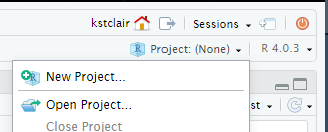
\includegraphics{img/maize_project.png}
  \item
    Select \textbf{Version Control} and then \textbf{New Project}
    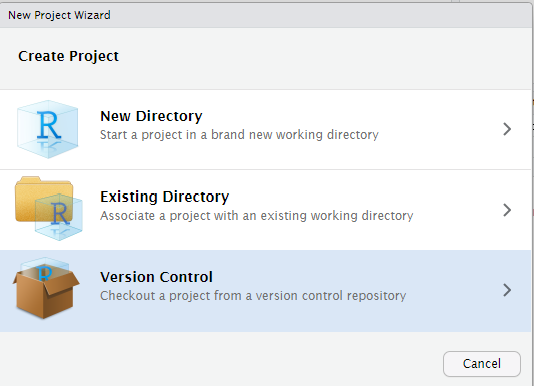
\includegraphics{img/maize_version.png}
    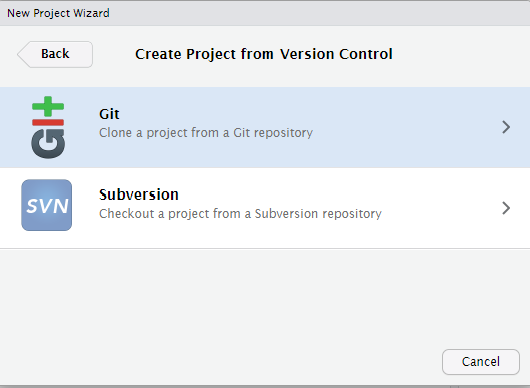
\includegraphics{img/maize_git.png}
  \item
    Paste the link you just copied into the Repository URL box. Leave
    the Project directory name blank (or keep the auto-filled name). Use
    the \textbf{Browse} button to find your \textbf{assignments} folder, then
    click \textbf{Create Project}
  \end{itemize}
\end{enumerate}

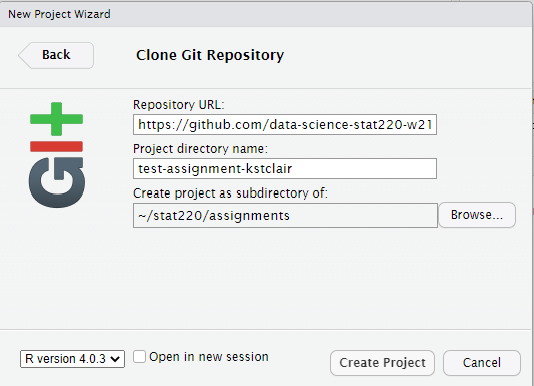
\includegraphics{img/maize_clone.png}

\hypertarget{working-on-your-assignment}{%
\subsection{Working on your assignment}\label{working-on-your-assignment}}

An RStudio project should now open, which will allow you to start
working on your homework assignment. You should see the project
assignment name in the top right side of Rstudio. You will probably see
a blank console screen when you open a new project. Look in the
\textbf{Files} tab for your homework .Rmd file. Click on whatever file you
want to edit (probably the .Rmd file) and edit away. Make sure that your
current assignment's project is the one open and showing in the upper
rightproject name. To \textbf{open} a project, click on the \texttt{.Rproj} file or
use the \textbf{Open Project\ldots{}} option available in the upper right project
link.

\hypertarget{commits}{%
\subsubsection{Commits}\label{commits}}

After you make changes to the homework assignment, commit them. What are
commits you ask? Commits are essentially taking a snapshot of your
projects. Commits save this snapshot to your local version of Git
(located on your hard drive or the maize server). For example, if I make
changes to a code so that it prints ``Hello world'', and then commit them
with an informative message, I can look at the history of my commits and
view the code that I wrote at that time. If I made some more changes to
the function that resulted in an error, I could go back to the commit
where the code was originally working. This prevents you from creating
several versions of your homework (homework-v1, homework-v2, \ldots) or
from trying to remember what your code originally looked like.

You can make commits in the Git tab in RStudio.

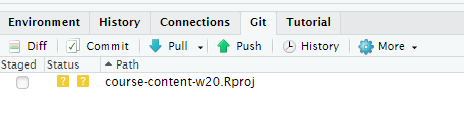
\includegraphics{img/maize_gittab.png}

Click the \textbf{Commit} button in the Git tab. Check the boxes of the files
that you want to commit, enter your commit message (briefly state what
changes have been made), then hit \textbf{Commit}. You can read how to do
this in RStudio in more detail here:
\url{http://r-pkgs.had.co.nz/git.html\#git-commit}.

Two things about committing.

\begin{itemize}
\tightlist
\item
  You should \textbf{commit somewhat frequently}. At minimum, if you're
  doing a homework assignment, you should make a commit each time that
  you've finished a question.
\item
  Leave \textbf{informative commit messages}. ``Added stuff'' will not help
  you if you're looking at your commit history in a year. A message
  like ``Added initial version of hello-world function'' will be more
  useful.
\end{itemize}

\hypertarget{pushing-changes-to-github}{%
\subsubsection{Pushing changes to Github}\label{pushing-changes-to-github}}

At some point you'll want to get the updated version of the assignment
back onto GitHub, either so that we can help you with your code or so
that it can be graded. You will also want to push work frequently when
you have a shared GitHub repo for project collaborations (i.e.~more than
one person is working on a project and code). If you are ready to push,
you can again click on the ``Up'' \textbf{Push} arrow in the Git tab or in the
Commit pop-up window or in the Git tab (shown above).

To ``turn in'' an assignment, all you need to do is push all your relevant
files to Github by the deadline.

\hypertarget{group-work}{%
\section{Group work}\label{group-work}}

Collaborative Github assignments are pretty similar to individual assignments.

\hypertarget{creating-a-grouppartner-assignment-repo-and-project}{%
\subsection{Creating a group/partner assignment repo and project}\label{creating-a-grouppartner-assignment-repo-and-project}}

Go to our course GitHub organization page(\href{https://github.com/DataScienceWinter24}{DataScienceWinter24}) and find the repo for your group, for example if your group name is ``team01'' the you might find the \texttt{mp1-team01} repo. Clone this repo to your computer/maize account using the same steps done for an individual assignment (see steps 2-3).

\hypertarget{working-with-collaborative-repos}{%
\subsubsection{Working with collaborative repos}\label{working-with-collaborative-repos}}

For group homework, I suggest that only the \emph{recorder} edit the group-homework-x.Rmd file to avoid merge conflicts! Other group members can create a new Markdown doc to run and save commands. Only the recorder needs to \textbf{push} changes (answers) to the Github repo and all others can then \textbf{pull} these changes (i.e.~the final answers) after the HW is submitted.

When you are working together on a Github project, you should commit and push your modifications frequently. You will also need to frequently \textbf{pull} updates from Github down to your local version of RStudio. These updates are changes that your teammates have made since your last pull. To pull in changes, click the ``Down'' \textbf{Pull} arrow in the Git tab (shown above).

If you get an error about conflict after pulling or pushing, don't freak out! This can happen if you edit a file (usually an .Rmd or .R file) in a location that was also changed by a teammate. When this happens you should attempt to fix the \textbf{merge conflict}. Take a look at \href{http://r-pkgs.had.co.nz/git.html\#git-pull}{this resource site} and try to fix the merge conflict in Rstudio.

\hypertarget{additional-resources}{%
\section{Additional resources}\label{additional-resources}}

\begin{itemize}
\tightlist
\item
  \href{http://happygitwithr.com/}{Happy Git and GitHub for the useR}
\item
  \href{http://r-pkgs.had.co.nz/git.html\#git-rstudio}{Rstudio, Git and GitHub}
\item
  \href{http://learngitbranching.js.org/}{Interactive learning guide for Git}
\item
  \href{https://guides.github.com/}{GitHub Guides}
\item
  \href{https://youtu.be/F_fPEMnr1OQ}{Git setup for Windows (video)}
\item
  \href{https://www.youtube.com/watch?v=kbmSZwK0k-A\&t}{Git setup for Mac (video)}
\item
  \href{https://youtu.be/pAcMgGbCtQw}{How to clone, edit, and push homework assignments with GitHub Classroom (video)}
\end{itemize}

\hypertarget{acknowledgements-1}{%
\section{Acknowledgements}\label{acknowledgements-1}}

Most of this content in this guide was taken from
\url{https://github.com/jfiksel/github-classroom-for-students}, edited for our classroom use by Katie St.~Clair.

\hypertarget{reuse}{%
\section{Reuse}\label{reuse}}

This guide is licensed under the CC BY-NC 3.0 Creative
Commons License.

\hypertarget{r-markdown-syntax}{%
\chapter{R Markdown Syntax}\label{r-markdown-syntax}}

Markdown is a simple formatting syntax for authoring HTML, PDF, and MS Word documents. For more details on using R Markdown see \url{http://rmarkdown.rstudio.com}.

\hypertarget{lists-in-r-markdown}{%
\subsection{Lists in R Markdown:}\label{lists-in-r-markdown}}

You can use asterisk mark to provide emphasis, such as \texttt{*italics*\ or\ **bold**}. You can create lists with a dash:

\begin{Shaded}
\begin{Highlighting}[]
\SpecialCharTok{{-}}\NormalTok{ Item }\DecValTok{1}
\SpecialCharTok{{-}}\NormalTok{ Item }\DecValTok{2}
\SpecialCharTok{{-}}\NormalTok{ Item }\DecValTok{3}
  \SpecialCharTok{+}\NormalTok{ Subitem }\DecValTok{1}
\SpecialCharTok{*}\NormalTok{ Item }\DecValTok{4}
\end{Highlighting}
\end{Shaded}

to produce

\begin{itemize}
\tightlist
\item
  Item 1
\item
  Item 2
\item
  Item 3

  \begin{itemize}
  \tightlist
  \item
    Subitem 1
  \end{itemize}
\item
  Item 4
\end{itemize}

You can embed Latex equations in-line, \texttt{\$\textbackslash{}frac\{1\}\{n\}\ \textbackslash{}sum\_\{i=1\}\^{}\{n\}\ x\_\{i\}\$} to produce \(\frac{1}{n} \sum_{i=1}^{n} x_{i}\) or in a new line as \texttt{\$\$\textbackslash{}text\{Var\}(X)\ =\ \textbackslash{}frac\{1\}\{n-1\}\textbackslash{}sum\_\{i-1\}\^{}\{n\}\ (x\_\{i\}\ -\ \textbackslash{}bar\{x\})\^{}2\$\$} to produce \[\text{Var}(X) = \frac{1}{n-1}\sum_{i-1}^{n} (x_{i} - \bar{x})^2\]

\hypertarget{embed-an-r-code-chunk}{%
\subsection{Embed an R code chunk:}\label{embed-an-r-code-chunk}}

Use the following

\begin{verbatim}
```r
Use back ticks to 
create a block of code
```
\end{verbatim}

to produce:

\begin{verbatim}
Use back ticks to 
create a block of code
\end{verbatim}

You can also evaluate and display the results of R code. Each tasks can be accomplished in a suitably labeled chunk like the following:

\begin{Shaded}
\begin{Highlighting}[]
\FunctionTok{summary}\NormalTok{(cars)}
\end{Highlighting}
\end{Shaded}

\begin{verbatim}
     speed           dist       
 Min.   : 4.0   Min.   :  2.00  
 1st Qu.:12.0   1st Qu.: 26.00  
 Median :15.0   Median : 36.00  
 Mean   :15.4   Mean   : 42.98  
 3rd Qu.:19.0   3rd Qu.: 56.00  
 Max.   :25.0   Max.   :120.00  
\end{verbatim}

\begin{Shaded}
\begin{Highlighting}[]
\NormalTok{fit }\OtherTok{\textless{}{-}} \FunctionTok{lm}\NormalTok{(dist }\SpecialCharTok{\textasciitilde{}}\NormalTok{ speed, }\AttributeTok{data =}\NormalTok{ cars)}
\NormalTok{fit}
\end{Highlighting}
\end{Shaded}

\begin{verbatim}

Call:
lm(formula = dist ~ speed, data = cars)

Coefficients:
(Intercept)        speed  
    -17.579        3.932  
\end{verbatim}

\hypertarget{including-plots}{%
\subsection{Including Plots:}\label{including-plots}}

You can also embed plots. See Figure \ref{fig:pie} for example:

\begin{Shaded}
\begin{Highlighting}[]
\FunctionTok{par}\NormalTok{(}\AttributeTok{mar =} \FunctionTok{c}\NormalTok{(}\DecValTok{0}\NormalTok{, }\DecValTok{1}\NormalTok{, }\DecValTok{0}\NormalTok{, }\DecValTok{1}\NormalTok{))}
\FunctionTok{pie}\NormalTok{(}
  \FunctionTok{c}\NormalTok{(}\DecValTok{280}\NormalTok{, }\DecValTok{60}\NormalTok{, }\DecValTok{20}\NormalTok{),}
  \FunctionTok{c}\NormalTok{(}\StringTok{\textquotesingle{}Sky\textquotesingle{}}\NormalTok{, }\StringTok{\textquotesingle{}Sunny side of pyramid\textquotesingle{}}\NormalTok{, }\StringTok{\textquotesingle{}Shady side of pyramid\textquotesingle{}}\NormalTok{),}
  \AttributeTok{col =} \FunctionTok{c}\NormalTok{(}\StringTok{\textquotesingle{}\#0292D8\textquotesingle{}}\NormalTok{, }\StringTok{\textquotesingle{}\#F7EA39\textquotesingle{}}\NormalTok{, }\StringTok{\textquotesingle{}\#C4B632\textquotesingle{}}\NormalTok{),}
  \AttributeTok{init.angle =} \SpecialCharTok{{-}}\DecValTok{50}\NormalTok{, }\AttributeTok{border =} \ConstantTok{NA}
\NormalTok{)}
\end{Highlighting}
\end{Shaded}

\begin{figure}
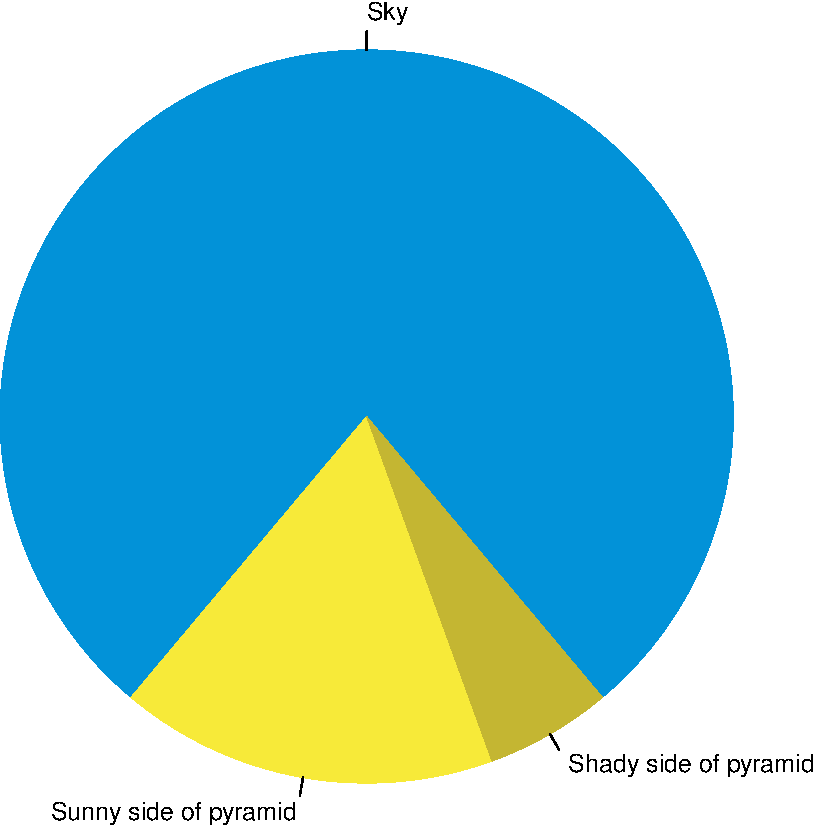
\includegraphics[width=1\linewidth]{rmarkdown_files/figure-latex/pie-1} \caption{A fancy pie chart.}\label{fig:pie}
\end{figure}

(Credit: Yihui Xie)

\hypertarget{read-in-data-files}{%
\subsection{Read in data files:}\label{read-in-data-files}}

\begin{Shaded}
\begin{Highlighting}[]
\NormalTok{simple\_data }\OtherTok{\textless{}{-}} \FunctionTok{read.csv}\NormalTok{(}\StringTok{"https://deepbas.io/data/simple{-}1.dat"}\NormalTok{, )}
\FunctionTok{summary}\NormalTok{(simple\_data) }
\end{Highlighting}
\end{Shaded}

\begin{verbatim}
   initials            state                age      
 Length:3           Length:3           Min.   :45.0  
 Class :character   Class :character   1st Qu.:47.5  
 Mode  :character   Mode  :character   Median :50.0  
                                       Mean   :52.0  
                                       3rd Qu.:55.5  
                                       Max.   :61.0  
     time          
 Length:3          
 Class :character  
 Mode  :character  
                   
                   
                   
\end{verbatim}

\begin{Shaded}
\begin{Highlighting}[]
\NormalTok{knitr}\SpecialCharTok{::}\FunctionTok{kable}\NormalTok{(simple\_data)}
\end{Highlighting}
\end{Shaded}

\begin{tabular}{l|l|r|l}
\hline
initials & state & age & time\\
\hline
vib & MA & 61 & 6:01\\
\hline
adc & TX & 45 & 5:45\\
\hline
kme & CT & 50 & 4:19\\
\hline
\end{tabular}

\hypertarget{hide-the-code}{%
\subsection{Hide the code:}\label{hide-the-code}}

If we enter the \texttt{echo\ =\ FALSE} option in the R chunk (see the .Rmd file). This prevents the R code from being printed to your document; you just see the results.

\begin{tabular}{l|l|r|l}
\hline
initials & state & age & time\\
\hline
vib & MA & 61 & 6:01\\
\hline
adc & TX & 45 & 5:45\\
\hline
kme & CT & 50 & 4:19\\
\hline
\end{tabular}

\hypertarget{github-tutorial}{%
\chapter{Github Tutorial}\label{github-tutorial}}

\begin{Shaded}
\begin{Highlighting}[]
\CommentTok{\# load the required libraries}
\FunctionTok{library}\NormalTok{(credentials) }\CommentTok{\# to help with PAT access}
\FunctionTok{library}\NormalTok{(gitcreds)}
\FunctionTok{library}\NormalTok{(usethis)}
\end{Highlighting}
\end{Shaded}

\begin{Shaded}
\begin{Highlighting}[]
\CommentTok{\# STEPS INVOLVED TO ESTABLISH GIT CREDENTIALS / PAT}

\CommentTok{\# Step 1}

\CommentTok{\# usethis::use\_git\_config(user.name = "deepbas", user.email = "deepbas99@gmail.com")}

\CommentTok{\# Step 2}

\CommentTok{\# usethis::create\_github\_token()}

\CommentTok{\# Step 3}

\CommentTok{\# if this is the second/subsequent iteration start from here}

\CommentTok{\# gitcreds::gitcreds\_set()}

\CommentTok{\# Verify}

\CommentTok{\# gitcreds::gitcreds\_get()}
\end{Highlighting}
\end{Shaded}

In this worksheet, you will practice creating a GitHub repository using the usethis::use\_github() function and cloning it back to your local machine using RStudio's menu options.

\hypertarget{tutorial-1-creating-and-cloning-a-repository-starting-from-github-to-rstudio}{%
\section{Tutorial 1: Creating and cloning a Repository starting from Github to RStudio}\label{tutorial-1-creating-and-cloning-a-repository-starting-from-github-to-rstudio}}

\begin{enumerate}
\def\labelenumi{\arabic{enumi}.}
\item
  Visit the GitHub website at \url{https://github.com} and sign in using your GitHub account. If you don't have an account yet, you can create one for free.
\item
  Once logged in, click on the ``+'' icon in the top right corner of the webpage, then click on ``New repository''.
\item
  Enter a name for your new repository in the ``Repository name'' field. You may also provide an optional description.
\item
  Choose the visibility of your repository by selecting either ``Public'' or ``Private''. Public repositories are visible to anyone, while private repositories are only visible to you and any collaborators you invite.
\item
  (Optional) Check the box to initialize the repository with a README file.
\item
  Click on the ``Create repository'' button to create your new repository.
\end{enumerate}

This will create a new GitHub repository on your Github account. Follow further to clone the repository to your local folder using RStudio.

\begin{enumerate}
\def\labelenumi{\arabic{enumi}.}
\item
  Go to your GitHub repository webpage and click on the green ``Code'' button. This will display a dropdown menu with a URL for your repository. Click on the clipboard icon to copy the URL to your clipboard.
\item
  Open RStudio, and from the ``File'' menu, select ``New Project''.
\item
  In the ``New Project'' dialog, choose ``Version Control''.
\item
  Select ``Git'' as the version control system.
\item
  In the ``Repository URL'' field, paste the URL that you copied from your GitHub repository webpage.
\item
  Choose a local directory where you want to clone the repository by clicking on the ``Browse'' button and navigating to the desired folder on your computer.
\item
  Click on ``Create Project'' to clone the GitHub repository to your local computer.
\end{enumerate}

\hypertarget{tutorial-2-creating-a-new-github-repository-using-usethis-r-package-rstudio-to-github-works-only-on-local-rstudio}{%
\section{\texorpdfstring{Tutorial 2: Creating a new GitHub repository using \texttt{usethis} R package (RStudio to Github) (Works ONLY on local RStudio)}{Tutorial 2: Creating a new GitHub repository using usethis R package (RStudio to Github) (Works ONLY on local RStudio)}}\label{tutorial-2-creating-a-new-github-repository-using-usethis-r-package-rstudio-to-github-works-only-on-local-rstudio}}

\hypertarget{prerequisites}{%
\subsection{Prerequisites}\label{prerequisites}}

\begin{enumerate}
\def\labelenumi{\arabic{enumi}.}
\item
  Install the usethis package if you haven't already: install.packages(``usethis'')
\item
  Make sure you have a GitHub account, and you are logged in.
\item
  Configure Git with your name and email address if you haven't already. Run the following commands in the R console, replacing ``Your Name'' and ``\href{mailto:youremail@example.com}{\nolinkurl{youremail@example.com}}'' with your information:
\end{enumerate}

\begin{Shaded}
\begin{Highlighting}[]
\NormalTok{usethis}\SpecialCharTok{::}\FunctionTok{use\_git\_config}\NormalTok{(}\AttributeTok{user.name =} \StringTok{"Your Name"}\NormalTok{, }\AttributeTok{user.email =} \StringTok{"youremail@example.com"}\NormalTok{)}
\end{Highlighting}
\end{Shaded}

\begin{enumerate}
\def\labelenumi{\arabic{enumi}.}
\setcounter{enumi}{3}
\item
  Create a new R project in RStudio by clicking on ``File'' \textgreater{} ``New Project'' \textgreater{} ``New Directory'' \textgreater{} ``New Project.'' Give your project a name and choose a location on your computer to save it. Click ``Create Project.''
\item
  Make a new file or copy and paste a .Rmd file that you want to have in your repo and save it to your requirement.
\end{enumerate}

\begin{enumerate}
\def\labelenumi{\arabic{enumi}.}
\setcounter{enumi}{5}
\tightlist
\item
  In the R console, load the usethis package:
\end{enumerate}

\begin{Shaded}
\begin{Highlighting}[]
\FunctionTok{library}\NormalTok{(usethis)}
\end{Highlighting}
\end{Shaded}

\begin{enumerate}
\def\labelenumi{\arabic{enumi}.}
\setcounter{enumi}{6}
\tightlist
\item
  Initialize a Git repository for your project by running:
\end{enumerate}

\begin{Shaded}
\begin{Highlighting}[]
\NormalTok{usethis}\SpecialCharTok{::}\FunctionTok{use\_git}\NormalTok{()}
\end{Highlighting}
\end{Shaded}

\begin{enumerate}
\def\labelenumi{\arabic{enumi}.}
\setcounter{enumi}{7}
\tightlist
\item
  Now, let's create a new GitHub repository using the usethis::use\_github() function. Run the following command:
\end{enumerate}

\begin{Shaded}
\begin{Highlighting}[]
\NormalTok{usethis}\SpecialCharTok{::}\FunctionTok{use\_github}\NormalTok{()}
\end{Highlighting}
\end{Shaded}

\begin{enumerate}
\def\labelenumi{\arabic{enumi}.}
\setcounter{enumi}{8}
\tightlist
\item
  Follow the instructions in the R console, and your GitHub repository will be created. Note the repository URL, as you will need it in the next activity.
\end{enumerate}

  \bibliography{book.bib,packages.bib}

\end{document}
